%\documentstyle[epsf,twocolumn]{jarticle}       %LaTeX2e仕様
\documentclass[twocolumn]{jarticle}     %pLaTeX2e仕様(platex.exeの場合)
% \documentclass[onecolumn]{ujarticle}   %pLaTeX2e仕様(uplatex.exeの場合)
%%%%%%%%%%%%%%%%%%%%%%%%%%%%%%%%%%%%%%%%%%%%%%%%%%%%%%%%%%%%%%
%%
%%  基本バージョン
%%
%%%%%%%%%%%%%%%%%%%%%%%%%%%%%%%%%%%%%%%%%%%%%%%%%%%%%%%%%%%%%%%%
\setlength{\topmargin}{-45pt}
%\setlength{\oddsidemargin}{0cm}
\setlength{\oddsidemargin}{-7.5mm}
%\setlength{\evensidemargin}{0cm}
\setlength{\textheight}{24.1cm}
%setlength{\textheight}{25cm}
\setlength{\textwidth}{17.4cm}
%\setlength{\textwidth}{172mm}
\setlength{\columnsep}{11mm}

%\kanjiskip=.07zw plus.5pt minus.5pt


% 【節が変わるごとに (1.1)(1.2) … (2.1)(2.2) と数式番号をつけるとき】
%\makeatletter
%\renewcommand{\theequation}{%
%\thesection.\arabic{equation}} %\@addtoreset{equation}{section}
%\makeatother

%\renewcommand{\arraystretch}{0.95} 行間の設定
%%%%%%%%%%%%%%%%%%%%%%%%%%%%%%%%%%%%%%%%%%%%%%%%%%%%%%%%
%\usepackage{graphicx}   %pLaTeX2e仕様(\documentstyle ->\documentclass)
\usepackage[dvipdfmx]{graphicx}
\usepackage{subcaption}
\usepackage{multirow}
\usepackage{amsmath}
\usepackage{url}
\usepackage{ulem}
\usepackage{algorithm}
\usepackage{algorithmic}
%%%%%%%%%%%%%%%%%%%%%%%%%%%%%%%%%%%%%%%%%%%%%%%%%%%%%%%%
\begin{document}

	%bibtex用の設定
	%\bibliographystyle{ujarticle}

	\twocolumn[
		\noindent
		\hspace{1em}
		2020 年 4 月 30 日
		ゼミ資料
		\hfill
		B4 杉山 竜弥
		\vspace{2mm}

		\hrule
		\begin{center}
			{\Large \bf 進捗報告}
		\end{center}
		\hrule
		\vspace{9mm}
	]

	% ‚ここから 文章 Start!
\section{今週やったこと}


\section{問題設定}
何を入力として何を出力とするかを明確に定義

	\subsection{}
	\subsubsection{}

		\begin{algorithm}
			\caption{Split Data Swap}
			\label{alg1}
			\begin{enumerate}{ % itemize, enumerate, description
				\item{データ 2N 抜き出す}
				\item{そのデータを N(A) と N(B)に分ける.}
				\item{A → train, B → test で実験}
				\item{B → train, A → test で実験}
				\item{3.と4.で test でミスしたデータを調べる}
				\item{A をテストとしたとき失敗したデータと B をテストとしたとき成功したデータを入れ替える.}
				\item{1.に戻る.}
			}\end{enumerate}
				% \begin{algorithmic}
				% \end{algorithmic}
		\end{algorithm}


\section{現在の状況}
何を使ってどのくらいの精度が出ているか?


\section{前回からの進捗}
あれば報告


\section{現在の問題点}
精度が出ない,とかだけではなく自分なりの考察を示す

\section{現在のソースコード}
埋め込みでもGitでもいいので参照できるように

\section{今後の予定}
なんとなくなんかの勉強をするとかではなく具体的に

	% \begin{figure}[htbp]
	% 	\begin{center}
	% 		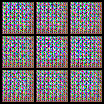
\includegraphics[clip,width=7.0cm]{../../test/images/0.png}
	% 	    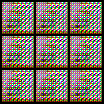
\includegraphics[clip,width=7.0cm]{../../test/images/3100.png}
	% 		\caption{学習結果 左:0 epoch, 右:1 epoch (32x32)}
	% 		\label{fig:result}
	% 	\end{center}
	% \end{figure}

	% 参考文献リスト
	\bibliographystyle{unsrt}
	\bibliography{ref}
\end{document}
